 \addtolength\abovedisplayskip{-1\baselineskip}%
  \addtolength\belowdisplayskip{-1\baselineskip}%
  
\begin{tikzpicture}
\node (datatitle) {\small Raw Data};
\node[below = -0.25cm of datatitle](data) {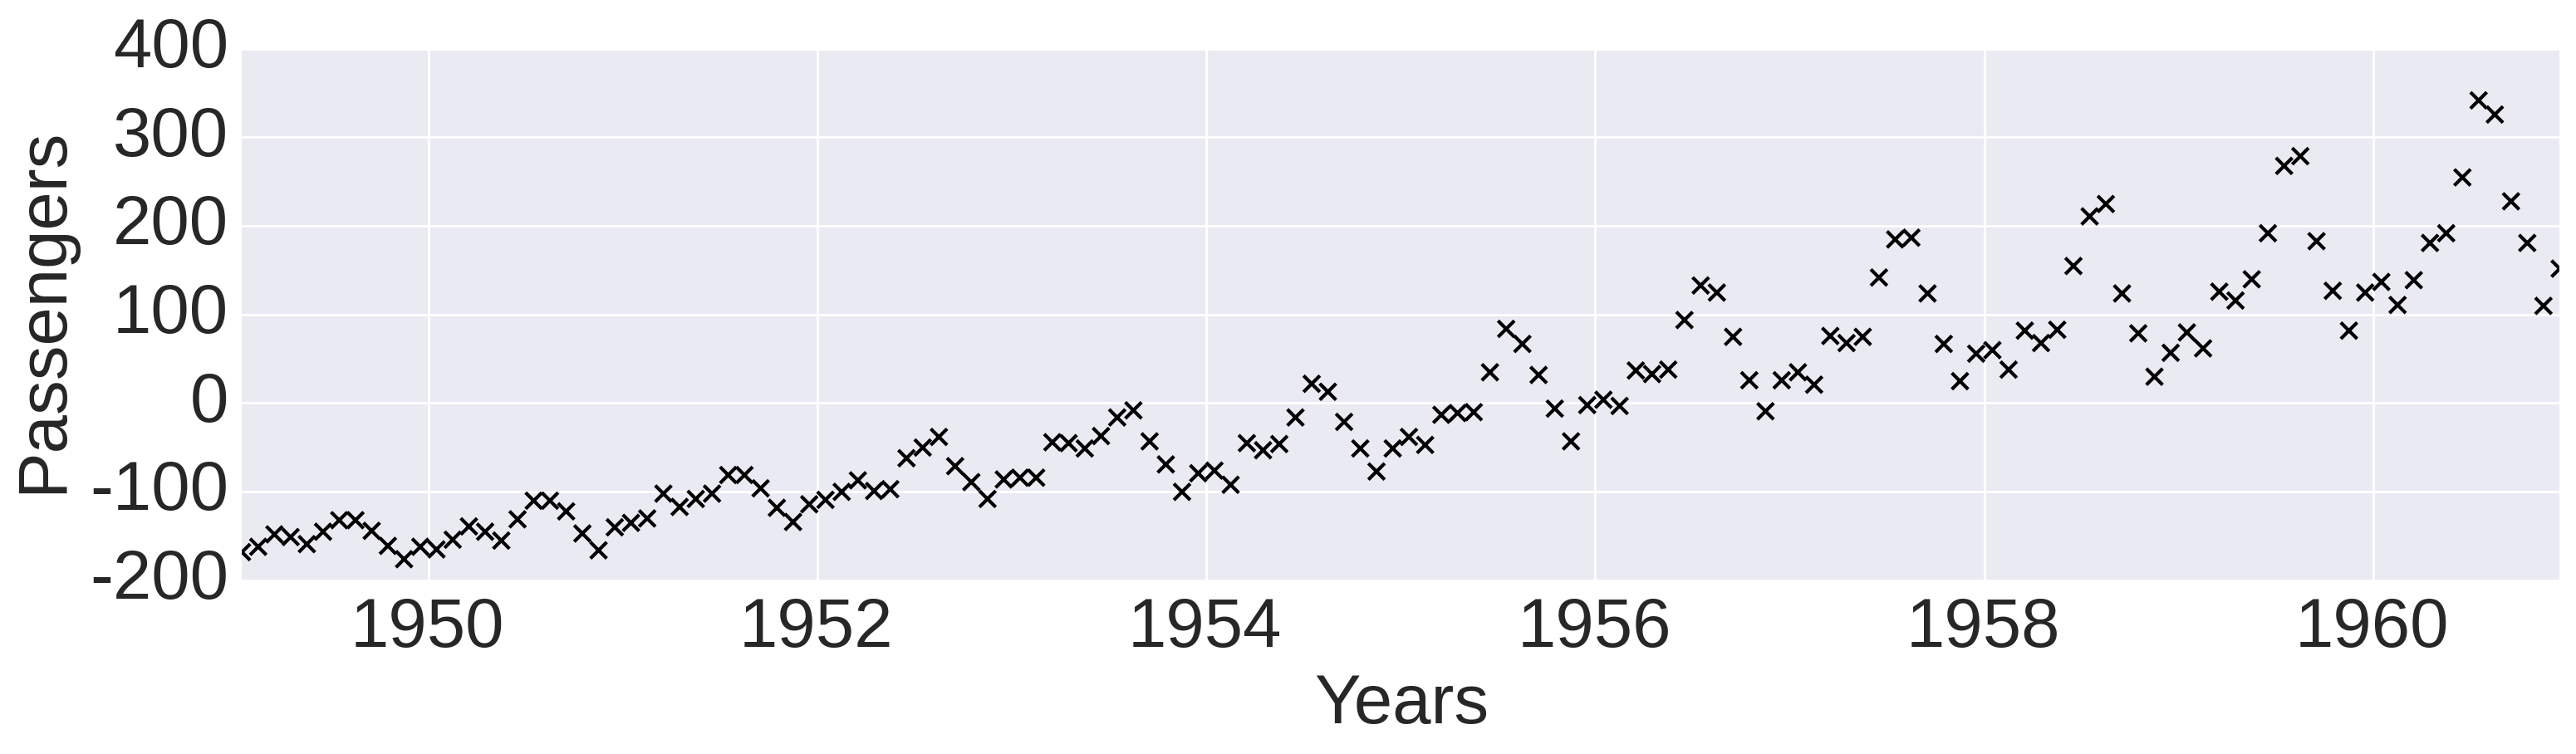
\includegraphics[width=0.65\textwidth]{figs/airline_data.png}};
\node[below= 1.2cm of data] (post_param) {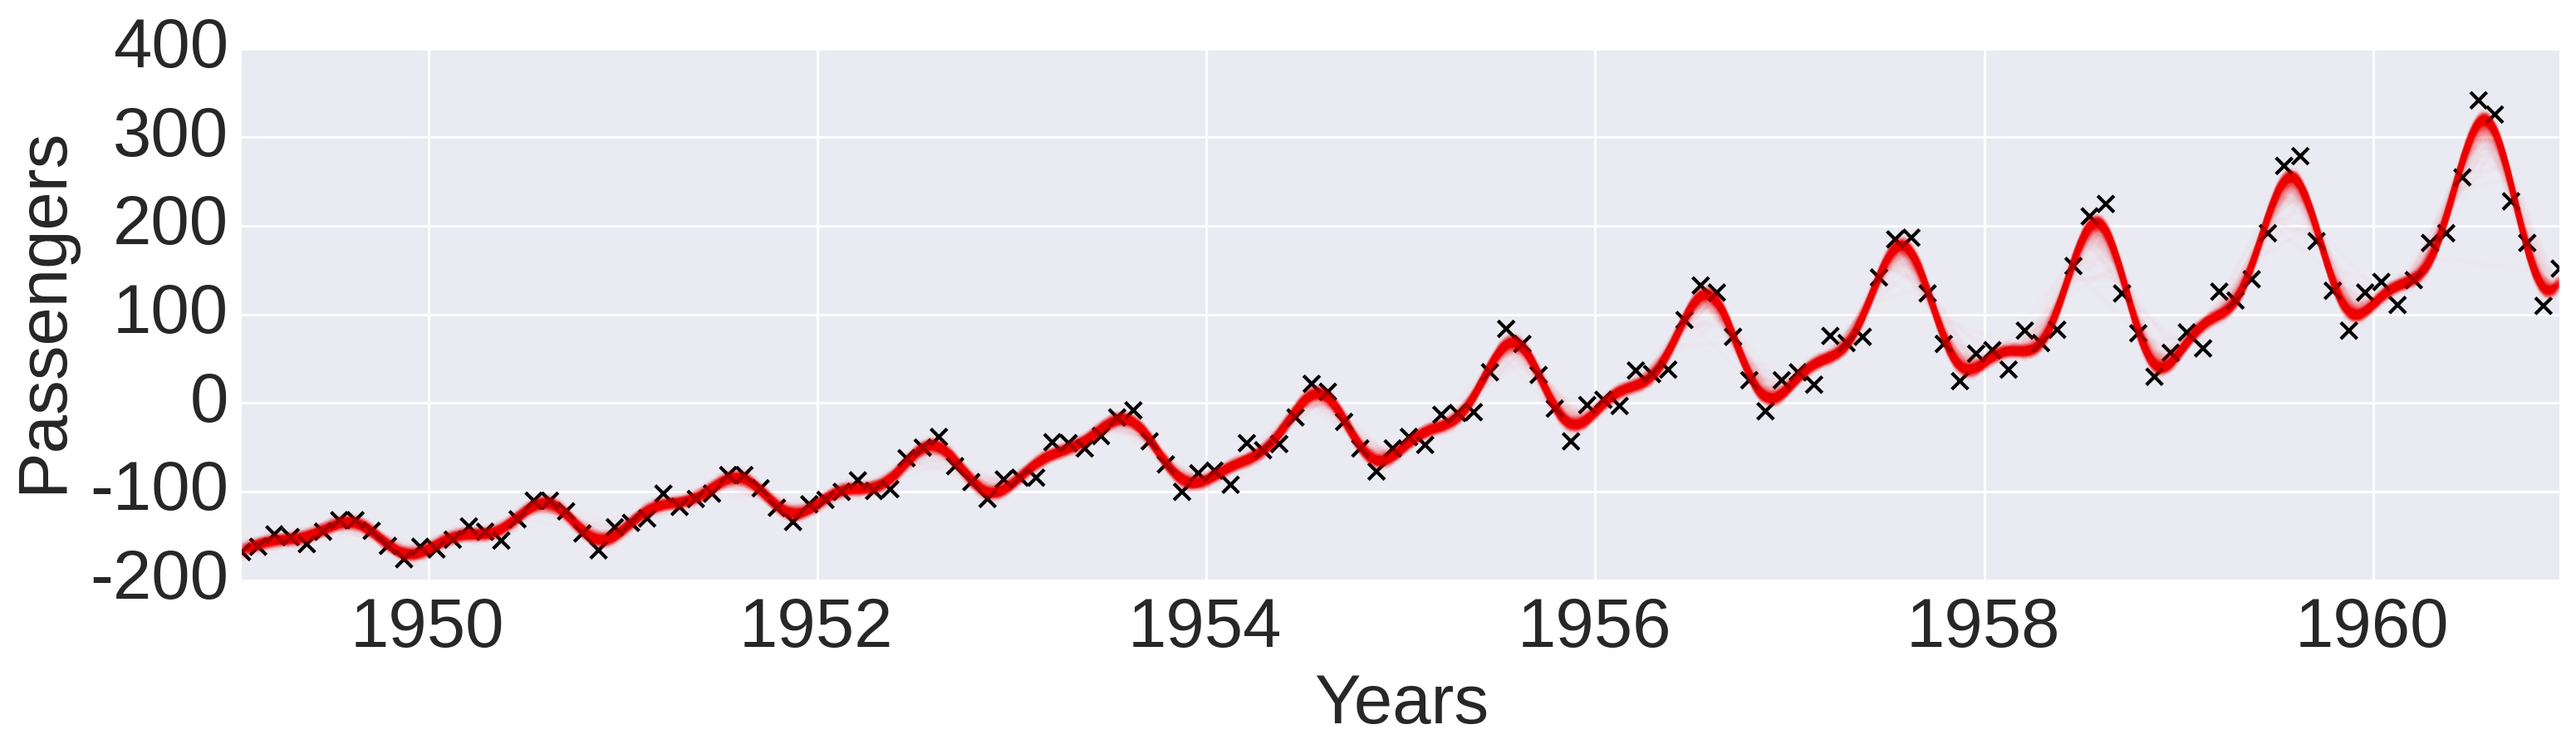
\includegraphics[width=0.65\textwidth]{figs/airline_sample_28.png}};


\node[below = 1.2cm of post_param] (posterior) {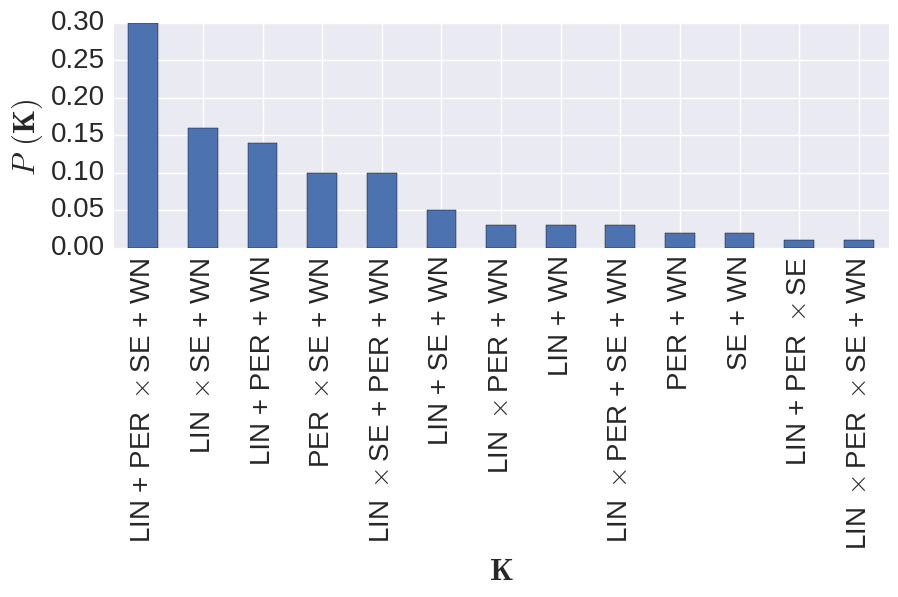
\includegraphics[width=0.55\textwidth]{figs/airline_structure.png}};


\node[draw,rectangle,below = 1.2cm of posterior] (formula_param_1) {\small\color{black}
$= 7.47^2(x x^\prime) +
\Bigg(0.27^2 \exp(-\frac{(x-x^\prime)^2}{2 \times 4.63^2}) \times 
7.34^2 \exp \bigg( \frac{2 \sin^2 ( \pi (x - x^\prime)/4.4}{4.55^2} \bigg)\Bigg)
+ 2.93^2 \delta_{x,x^\prime} \label{eq:WN}$ };


\node[draw,rectangle,below = 1.2cm of formula_param_1,text width =0.9\textwidth,minimum height = 1.5cm, font=\footnotesize] (paragraph){ 
The posterior peaks at a kernel structure with three additive components. Additive components hold globally, that is there are no higher level, qualitative aspects of the data that vary with the input space. The additive components are as follows: (i) a linearly increasing function or trend; (ii) a approximate periodic function; and (iv) white noise.};







\node[draw, rectangle, left = -1.7cm of posterior,minimum width = 0.45cm, minimum height = 5.2cm,yshift=0.2cm] (mark_structure) {};
%\node[draw,very thick, rectangle, below = 1.1cm of data,minimum width = \textwidth, minimum height = 15cm] (posterior_frame) {};

%\node[left = 1.3cm of mark_structure] (paragraph_helper){};
\node[below =0.45cm of mark_structure,inner sep = 0pt,outer sep=0pt] (formula_helper) {};
\node[above =1.2cm of formula_param_1,inner sep = 0pt,outer sep=0pt] (formula_helper_2) {};

%\draw[-,dashed] (mark_structure.south) -- (formula_helper);
%\draw[-,dashed] (formula_helper) -- (formula_helper_2);
%\draw[->,dashed] (mark_structure) -- (paragraph_helper);
%\draw[->,dashed] (formula_helper_2) -- (formula);

\draw[->] (data) -- node[right]{\small $\hat \fbf \sim
\mathcal{N}(\hat{\bm{\mu}},\hat\Kbf)$} (post_param_helper_1);
\draw[->] (post_param_helper_2) -- node[right]{\small Marginal Structure} (posterior);
\draw[->] (formula_helper_2) -- node[right] {\small
$\bm{\theta}=\{7.47,0.27,4.63,7.34,4.4,4.55,2.93\}$} (formula_param_1);
\draw[-] (mark_structure) -- node[left, yshift=-0.3cm] {\small $\Ktheta$} (formula_helper);
\draw[-] (formula_helper) --(formula_helper_2);
\draw[->] (formula_param_1) -- node[right]{\small Qualitative Interpretation} (paragraph);


\node[left=0.3cm of paragraph] (e){(e)}; 

\node[above=1.9cm of e] (d) {(d)}; 
\node[above=5.0cm of d] (c) {(c)}; 
\node[above=4.7cm of c] (b) {(b)}; 
\node[above=4.0cm of b] (a) {(a)}; 
\end{tikzpicture}
\addtolength\abovedisplayskip{1\baselineskip}%
\addtolength\belowdisplayskip{1\baselineskip}%


